% Preamble -----------------------------------------------------------------------------

\documentclass[12pt]{article}

    \usepackage[utf8]{inputenc}
    \usepackage{xcolor}
    \usepackage{amsmath,amsfonts,amssymb}
    \usepackage[english,spanish]{babel}
    \usepackage[left=2.00cm, right=2.00cm, top=2.00cm, bottom=2.00cm]{geometry}
    \usepackage{float}
    \usepackage{graphicx, graphics}
    \usepackage{hyperref}
    \linespread{1.5}
    \usepackage{multicol}
    \usepackage{hyperref}
    
% Document ----------------------------------------------------------------------------
\begin{document}

    \begin{flushleft}
        \vspace{6cm}
        {\huge \textbf{Solución de la ecuación de Schr\"odinger para el átomo de hidrógeno en coordenadas esferoidales prolatas}}\\
        \vspace{2mm}
        {\Large H. Celemin \footnote{Departamento de Matemáticas y Estadística, Universidad del Tolima},E. J. Machado\footnote{Departamento de Matemáticas y Estadística, Universidad del Tolima},J.A. Cardona Bedoya\footnote{Departamento de Física, Universidad del Tolima}}
    \end{flushleft}

    \begin{otherlanguage}{spanish}
        \begin{abstract}
            El sistema de coordenadas esferoidales prolatas $(\xi ,\eta,\phi)$ es ortogonal y es el 
            resultado de la rotación de una elipse alrededor de su eje mayor (eje en el cual 
            los focos están situados). El átomo de hidrógeno como sistema atómico más 
            sencillo es resuelto usando coordenadas esferoidales prolatas. Considerando que 
            el núcleo del átomo de hidrogeno está ubicado en uno de los focos de la elipse, se 
            encuentra que la ecuación de Schr\"odinger es separable en dichas coordenadas 
            $\left(\Psi(\xi,\eta,\phi) = X(\xi)Y(\eta)\Phi(\phi)\right)$. Con el fin de facilitar los cálculos se supone que 
            la distancia entre el centro de la elipse y el foco es un número semi-entero del 
            radio de Bohr ($\textbf{a}_{0}$), con esta suposición se encuentra una expresión para la 
            función de onda $\Psi(\xi,\eta,\phi)$ del átomo de hidrogeno \\
            \textbf{Palabras clave:} \hspace{1mm} \textit{átomo de hidrógeno.}
        \end{abstract}
    \end{otherlanguage}

    \begin{otherlanguage}{english}
        \begin{abstract}
            The prolate spheroidal coordinates system $(\xi ,\eta,\phi)$ is orthogonal and results 
            from rotating of an ellipse the about the major axis of the ellipse, i.e., the axis 
            on which the foci are located. The hydrogen atom as atomic simpler system is 
            solved using prolate spheroidal coordinates. Considering that the nucleus of 
            the hydrogen atom is located on one of the foci of the ellipse, the Schrödinger 
            equations is separable in these coordinates $\left(\Psi(\xi,\eta,\phi) = X(\xi)Y(\eta)\Phi(\phi)\right)$.In 
            order to facilitate the calculations we assumed that the distance between the 
            center of the ellipse and the focus is a semi-entire number of Bohr’s radius ($\textbf{a}_{0}$), 
            with this supposition we find an expression for the wave function $\Psi(\xi,\eta,\phi)$ of the hydrogen atom.\\
            \textbf{Key Words:} \hspace{1mm} \textit{hydrogen atom}
        \end{abstract}
    \end{otherlanguage}

    \newpage
    %\begin{multicols}{2}
        %% Section 1
        \section{Introducción}
        {\Huge L}a Física teórica posee dos herramientas 
        importantes: el tratamiento matemático 
        expresado con mucha frecuencia en 
        forma de una ecuación diferencial, y como este 
        tratamiento puede ser reflejado en función de 
        las reglas que rigen un fenómeno físico. El 
        problema netamente matemático del átomo 
        de hidrógeno ha sido ampliamente estudiado 
        y fue de gran interés para la teoría atómica. 
        Este átomo es el mas simple de los átomos, ya 
        que contiene solamente un electrón orbitando 
        alrededor de un núcleo muy masivo; la 
        ecuación de Schrödinger de este sistema se ha 
        solucionado en los sistemas de coordenadas 
        esféricas y parabólicas \textcolor{blue}{\cite{Schiff,Landau}}.

        Las coordenadas esferoidales prolatas han 
        sido utilizadas ampliamente en una diversidad 
        de trabajos en todas las áreas de la física, ya 
        que permite modelar sistemas con simetría 
        axial \textcolor{blue}{[3-5]} % \textcolor{blue}{\cite{Comasb,León,Quevedo}} genera un error al compilar
        .Lo anterior ha motivado la 
        utilización de este sistema de coordenadas no 
        convencional para solucionar la ecuación de 
        Schr\"odinger del átomo de hidrógeno.

        En la siguiente sección se presenta el modelo 
        teórico utilizado para solucionar la ecuación 
        de Schr\"odinger del átomo de Hidrogeno en 
        coordenadas esferoidales prolatas, y se hace 
        una descripción breve de estas coordenadas. 
        En la sección tres se presentan los desarrollos 
        matemáticos, y se obtienen las soluciones de 
        las ecuaciones diferenciales que provienen 
        de la separación de variables de la ecuación 
        de Schr\"odinger. Finalmente se presentan las conclusiones.

        %% Section 2
        \section{Modelo teórico aplicado}
        La mayor complejidad del átomo de 
        hidrógeno para la aplicación de la ecuación de 
        Schr\"odinger es la presencia de dos partículas 
        el núcleo y el electrón. Por ello es preciso 
        crear un sistema modelado donde se considera 
        el núcleo de carga positiva fijo en uno de
        los focos de la elipse con masa infinita y el 
        electrón moviéndose a su alrededor con masa 
        reducida $m$ (\textcolor{blue}{figura \ref{Figura 1}}). Se supone que la órbita 
        del electrón es de tipo esferoidal prolata. Las 
        coordenadas más adecuadas para describir 
        este modelo son las coordenadas esferoidales 
        prolatas ($\xi, \eta, \phi$) definidas así:
        %%% Equation 1
        \begin{equation}\label{Equation 1}
            \xi = \dfrac{(r_{1} + r_{2})}{2a}, \eta = \dfrac{(r_{1} + r_{2})}{2a}, \phi = \phi,
        \end{equation}
        donde $r_{1}$ y $r_{2}$ son las distancias desde 
        cualquier punto a los focos de la elipse, 
        separados por la distancia $2a$. 
        %%% Figura 1
        \begin{figure}[H] 
            \centering
            \caption{Átomo de hidrógeno en el modelo propuesto}
            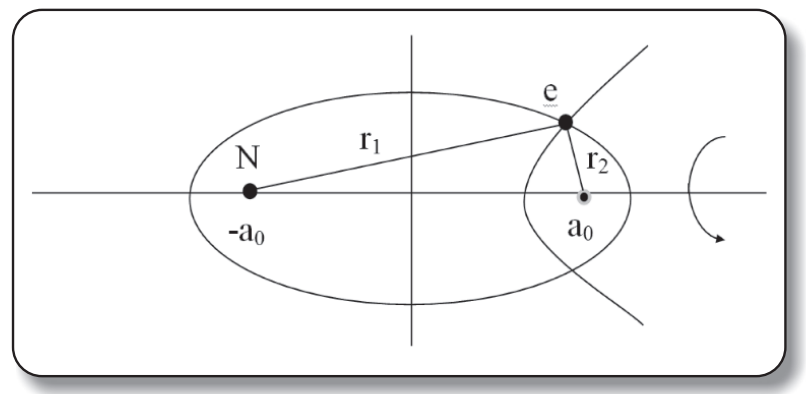
\includegraphics[scale=0.4]{Figuras/Figura1.PNG}
            \label{Figura 1}
        \end{figure}
        La (\textcolor{blue}{figura \ref{Figura 2}}) muestra las coordenadas 
        esferoidales prolatas (Fuente: Mathematical 
        Methods for Physicists, 2nd ed. Orlando, 
        Academic Press, pp. 93, 1971). En estas 
        coordenadas, $\eta$ define una familia de 
        hiperboloides de revolución alrededor de $z$, 
        mientras que $\xi$ define una familia de elipsoides 
        de revolución alrededor de $z$, con una distancia 
        interfocal $2a$ y la coordenada es el ángulo de 
        azimutal \textcolor{blue}{\cite{Arfken}}. 
        %%% Figura 2
        \begin{figure}[H] 
            \centering
            \caption{Coordenadas esferoidales prolatas}
            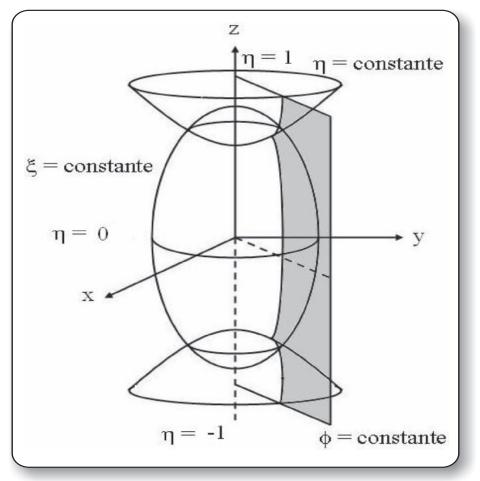
\includegraphics[scale=0.5]{Figuras/Figura2.PNG}
            \label{Figura 2}
        \end{figure}
        %%% Equation 2 y 3
        \begin{eqnarray}
            \xi &=& \text{constante}, \, \, \, -1 < \eta < 1, \, \, \, \, 0 \leq \phi \leq 2\pi \label{Equation 2}\\
            \eta &=& \text{constante}, \, \, \, -1 < \xi < \infty, \, \, \, 0 \leq \phi \leq 2\pi \label{Equation 3}
        \end{eqnarray}
        Para la descripción de nuestro modelo, la 
        ecuación de Schr\"odinger viene dada por:
        %%% Equation 4
        \begin{equation}\label{Equation 4}
            -\dfrac{\hbar^{2}}{2m} \nabla^{2} \psi \left(\xi,\eta,\phi\right)-\dfrac{e^{2}}{4\pi\varepsilon_{0}r_{1}}\Psi\left(\xi,\eta,\phi\right) = E\Psi \left(\xi,\eta,\phi\right),
        \end{equation}
        donde m es la masa reducida del sistema, $r_{1}$
        es la distancia entre el núcleo y el electrón. 
        En coordenadas esferoidales, el Laplaciano 
        tiene la forma de \textcolor{blue}{\cite{Morse}}:
        %%% Equation 5
        \begin{equation}\label{Equation 5}
            \nabla^{2}\Psi = \dfrac{1}{a^{2}\left(\xi^{2}-\eta^{2}\right)}\left[\dfrac{\partial}{\partial \xi}\left(\xi^{2}-1\right)\dfrac{\partial}{\partial \xi} + \dfrac{\partial}{\partial \eta}\left(1-\eta^{2}\right)\dfrac{\partial}{\partial \eta} + \dfrac{\xi^{2}-\eta^{2}}{\left(\xi^{2}-1\right)\left(1-\eta^{2}\right)} \dfrac{\partial^{2}}{\partial \phi^{2}} \right]\Psi
        \end{equation}
        La distancia $r_{1}$ entre el núcleo y el electrón 
        expresada en coordenadas esferoidales prolatas 
        vienen dada por: $r_{1} = a\left(\xi + \eta\right)$ Sustituyendo esta expresión en la ecuación 4, se obtiene:
        %%% Equation 6
        \begin{equation}
            -\nabla^{2}\Psi\left(\xi,\eta,\phi\right) - \dfrac{2me^{2}}{4\pi\varepsilon_{0}\hbar^{2}}\dfrac{1}{a\left(\xi + \eta\right)}\Psi\left(\xi, \eta,\phi\right) - \dfrac{2mE}{\hbar^{2}}\Psi\left(\xi,\eta,\phi\right) = 0
        \end{equation}
        Para la solución de la ecuación de 
        Schr\"odinger, es conveniente usar el radio 
        de Bohr: $a_{0}=4\pi\varepsilon_{0}\hbar^{2}/e^{2}m$ y considerar 
        que $\in^{2} = 2mE/\hbar^{2}$, además se supone que la 
        distancia entre el centro de la elipse y el foco 
        es un número semi-entero del radio de Bohr 
        ($a = a_{0}/\ell $, $\ell$ entero). Considerando esto, la 
        ecuación anterior se transforma en:
        %%% Equation 7
        \begin{equation}\label{Equation 7}
            \nabla^{2}\Psi\left(\xi, \eta, \phi\right) + \dfrac{2\ell}{a_{0}^{2}}\dfrac{1}{\left(\xi + \eta\right)}\Psi\left(\xi,\eta,\phi\right) + \in^{2}\Psi\left(\xi,\eta,\phi\right) = 0
        \end{equation}
        
        %% Section 3
        \section{Función de onda}
        La ecuación anterior es separable. 
        Escribiendo $\Psi\left(\xi,\eta,\phi\right) = X\left(\xi\right)Y\left(\eta\right)\Phi\left(\phi\right)$, y 
        sustituyendo esta expresión en la ecuación 
        \eqref{Equation 7} , se obtienen las siguientes ecuaciones 
        diferenciales
        %%% Equation 8,9 y 10
        \begin{eqnarray}
            \dfrac{d^{2}\Phi (\phi)}{d\phi^{2}} &=& -m^{2}\Phi(\phi), \label{Equation 8} \\
            \dfrac{d}{d\xi}\left(\xi^{2}-1\right)\dfrac{dX(\xi)}{d\xi} - \left(\dfrac{m^{2}}{\xi^{2}-1}-\dfrac{2\xi}{\ell}-\dfrac{a_{0}^{2}}{\ell^{2}}\in^{2}\xi^{2}\right)X(\xi) &=& kX(\xi), \label{Equation 9} \\
            \dfrac{d}{d\xi}\left(\eta^{2}-1\right)\dfrac{dY(\eta)}{d\eta} - \left(\dfrac{m^{2}}{\eta^{2}-1}-\dfrac{2\eta}{\ell}-\dfrac{a_{0}^{2}}{\ell^{2}}\in^{2}\eta^{2}\right)Y(\eta) &=& kY(\eta), \label{Equation 10}
        \end{eqnarray}
        donde $k$ es la constante de acoplamiento 
        entre las dos últimas ecuaciones. La ecuación 
        \eqref{Equation 8} tiene como solución
        %%% Equaion 11  
        \begin{equation} \label{Equation 11}
            \Phi(\phi) = \dfrac{1}{\sqrt{2\pi}}exp(im\phi), \, \, \, m = 0, \pm 1, \pm 2, \pm 3, \dots 
        \end{equation}
        donde $m$ es el número cuántico orbital. 
        Como las ecuaciones \eqref{Equation 9} y \eqref{Equation 10} son las mismas, 
        basta con resolver una de ellas. El punto $\xi = 1$ 
        en la ecuación \eqref{Equation 9} es un punto regular singular, 
        y es removible, de tal manera que la solución 
        es de la forma \textcolor{blue}{\cite{Tijonov}}:
        %%% Equation 12
        \begin{equation}\label{Equation 12}
            X(\xi) = \left(\xi^{2}-1\right)^{|m|/2}P(\xi),
        \end{equation}
        donde la función $P(\xi)$ satisface la ecuación:
        %%% Equation 13
        \begin{equation}\label{Equation 13}
            \left(\xi^{2}-1\right)\dfrac{d^{2}P(\xi)}{d\xi^{2}} + 2\left(|m| + 1\right)\xi \dfrac{dP(\xi)}{d\xi} + \left(|m| + m^{2} + \dfrac{2\xi}{\ell} + \dfrac{a_{0}^{2}}{\ell^{2}}\in^{2}\xi^{2} + k\right)P(\xi) = 0
        \end{equation}
        Realizando un cambio conveniente de la 
        variable independiente, $\xi = (\zeta + 1)/(\zeta - 1)$ \textcolor{blue}{\cite{Jaffe}}
        en la ecuación anterior y considerando que 
        $P(\xi) = Q(\zeta)$ se obtiene:
        %%% Equation 14
        \begin{equation*}
            \zeta(1-\zeta)^{4}\dfrac{d^{2}Q(\zeta)}{d\zeta^{2}} + \left[\left(|m| - 1\right)\zeta + \left(|m| + 1\right)\right](1-\zeta)^{3}\dfrac{dQ(\zeta)}{d\zeta} 
        \end{equation*}
        \begin{equation}\label{Equation 14}
            + \left[ (|m|+m^{2} + k)(1-\zeta)^{2}+\left(\frac{2}{\ell}\right)(1-\zeta^{2}) + \left(\dfrac{a_{0}^{2}\in^{2}}{\ell^{2}}\right)(1+\zeta)^{2} + 2\ell (1-\zeta^{2}) \right]  Q(\zeta) = 0
        \end{equation}
        La solución en series de potencia
        $Q(\zeta) = \sum\limits_{n=0}^{\infty}b_{n}\zeta^{n} $, es sustituida en la ecuación (14), 
        obteniendo la relación de recurrencia:
        %%% Equation 15
        \begin{equation}\label{Equation 15}
            \alpha_{n}b_{n+1} + \beta_{n}b_{n} + \gamma_{n}b_{n-1} + \delta_{n}b_{n-2} +\varepsilon_{n}b_{n-3} = 0
        \end{equation}
        donde,
        %%% Equation 16, 17, 18, 19 y 20
        \begin{eqnarray}
            \alpha_{n} &=& \left(n+1\right)\left(n+1+|m|\right), \label{Equation16}\\
            \beta_{n} &=& -2n\left(2n+|m|\right) + m^{2}+|m| + k + \dfrac{a_{0}\in^{2}}{\ell^{2}}+\dfrac{2}{\ell}, \label{Equation 17}\\
            \gamma_{n} &=& 6(n-1)^{2}-2\left(m^{2} + |m| + k + \dfrac{a_{0}^{2}\in^{2}}{\ell^{2}}\right), \label{Equation 18} \\
            \delta_{n} &=& 2(n-2)\left(|m| - 2n + 4\right) + m^{2} + |m| + k + \dfrac{a_{0}\in^{2}}{\ell^{2}}-\dfrac{2}{\ell}, \label{Equation 19}\\
            \varepsilon_{n} &=& (n-3)\left(n-3-|m|\right), \label{Equation 20}
        \end{eqnarray}
        y se toma $b_{0} = 1$. Esto permite generar todos 
        los coeficientes $b_{n}$
        de la serie de potencia, 
        consecuentemente la solución de la ecuación 
        \eqref{Equation 14} es obtenida.

        Conociendo las soluciones de las ecuaciones 
        diferenciales \eqref{Equation 8}, \eqref{Equation 9} y \eqref{Equation 10} se encuentra que la 
        función de onda en coordenadas esferoidales 
        prolatas viene dada por:
        %%% Equation 21
        \begin{equation}
            \Psi_{n_{1}n_{2}m}\left(\xi,\eta,\eta\right) = \dfrac{1}{\sqrt{2\pi}}\left(\xi^{2}-1\right)^{|m|/2}\sum\limits_{n_{1} = 0}^{\infty}\left(\dfrac{\xi-1}{\xi+1}\right)^{n_{1}} \left(\eta^{2}-1\right)^{|m|/2}\sum\limits_{n_{2} = 0}^{\infty}c_{n_{2}}\left(\dfrac{\eta-1}{\eta +1}\right)^{n_{2}}exp(im\phi)
        \end{equation}
        De tal forma que cada estado estacionario del 
        espectro discreto se determina en coordenadas 
        esferoidales prolatas por tres números enteros: 
        $m$ (número cuántico orbital) y 
        $n_{1}$, $n_{2}$(números cuánticos esferoidales prolatas).

        %% Section 4
        \section{Conclusiones}
        En este trabajo se ha encontrado la 
        función de onda para el átomo de hidrógeno 
        en coordenadas esferoidales prolatas, 
        considerando que la distancia entre el centro 
        del elipsoide y uno de sus focos es un número 
        semientero del radio de Bohr.

        %% Referencias
        \begin{thebibliography}{10}
            \bibitem{Schiff} L. I. Schiff, Quantum Mechanics,McGraw-Hill Book Company,New York1968
            \bibitem{Landau} L. D. Landau, E. M. Lifshitz, Mecánica Cuántica No-Relativista,Reverte,Barcelona, 1967
            \bibitem{Comasb} F. Comasb, Nelson Studarta and G. E. Marques, Solid State Commun, 130, 447, (2004)
            \bibitem{León} H. León, , J.L. Marín and R. Riera, Physica E, 27, 385 (2005)
            \bibitem{Quevedo} H..Quevedo, Phys. Rev. D 39, 2904 (1989)
            \bibitem{Arfken} G. Arfken, Mathematical Methods for Physicists. Academic Press, 1971.
            \bibitem{Morse} P. M. Morse and H. Fesbach, Methods of Theoretical Physics. McGraw-Hill, New York, 1953
            \bibitem{Tijonov} A. N. Tijonov, y A: A. Samarsky, A.A. Ecuaciones de la Física Matemática. Mir, 1980.
            \bibitem{Jaffe} G. Jaffe, Z. Physik 87, 535 (1934)
        \end{thebibliography}

    %\end{multicols}
\end{document}
